% Chapter 3

\chapter{Chapitre 4 : BSO pour le problème de recherche de cibles} % Main chapter title

\label{Chapter4} % For referencing the chapter elsewhere, use \ref{Chapter1} 
%----------------------------------------------------------------------------------------
\section{Introduction}
Dans ce chapitre, nous présentons notre approche de résolution basée sur l’algorithme BSO. Dans un premier temps, le robot simule le comportement d’une seule abeille alors que dans une seconde implémentation, le robot simule tout un essaim d’abeilles, l’approche dans ce cas est appelée Multi-BSO. Le principe de fonctionnement de chaque algorithme, à savoir BSO, Multi-BSO sera détaillé.

Un récapitulatif du travail effectué et de son importance pour la phase d’implémentation clôtura ce chapitre.




\section{Mono-BSO \textit{vs} Multi-BSO}
Les robots constituent un seul groupe qui simule le comportement des abeilles. Il existe donc une communication de type stigmergique entre les robots, concrétisée à l’aide de la simulation de la danse des abeilles. Ce qui amène à déduire qu’il existe une intelligence collective entre les robots déployés et qu'ils interagissent de manière coopérative pour la recherche des cibles.

Nos deux approches BSO et Multi-BSO reposent certes toutes les deux sur les mêmes concepts de base, mais sont utilisées de manières bien différentes, telles que pour :  
\paragraph{- Mono-BSO,}chaque robot se comporte comme une seule abeille. Il occupe une case ayant une certaine position dans l’environnement et peut tester la qualité de sa position en tant que solution, grâce à la fonction objectif.

\paragraph{- Multi-BSO,}comme son nom l’indique consiste en l’application de BSO par plusieurs essaims d’abeilles. Dans ce cas, chaque robot se comporte comme un essaim d’abeilles lui permettant de se déplacer à la recherche d'une solution optimale. 




\section{Adaptation de BSO pour le problème de la recherche de cibles}
Au deuxième chapitre, nous avons exposé l’algorithme générique BSO pour la résolution d’un problème complexe quelconque. Dans cette section, nous nous intéressons à son application au problème de la recherche de cibles. Chaque composant spécifique à l’algorithme comme la solution, la fonction objectif, le paramètre Flip et la table Dance sera adapté à ce problème.

\subsection{Solution}
Une solution est la position de coordonnées \textit{(x, y)} dans laquelle se trouve une abeille. Cette position correspond à une case ayant une certaine valeur.

\subsection{Fonction objectif}
Chaque abeille est responsable de l'évaluation de sa solution, en vérifiant la valeur contenue  dans la case où elle se trouve. Si une cible est détectée la valeur trouvée est alors de 1. 

\subsection{Flip} Il s'agit du paramètre de diversification. Dans l'environnement que nous traitons pour ce problème, le \textbf{flip} permet de déterminer la zone de recherche globale à partir d'une position initiale \textit{I}, cela à travers le calcul des positions à une distance \textit{R} (rayon) de la position initiale.

\begin{equation}
\label{eq:flip}
R = Taille_{Cot\acute{e}} / flip 
\end{equation}
Avec:
$Taille_{Cot\acute{e}}$ : Taille du coté de l'environnement.\\

Les positions générées constituent le cercle de rayon \textit{R} ayant pour centre la position initiale \textit{I}. La figure \ref{flip} schématise ce processus.\\

\begin{center}	  
	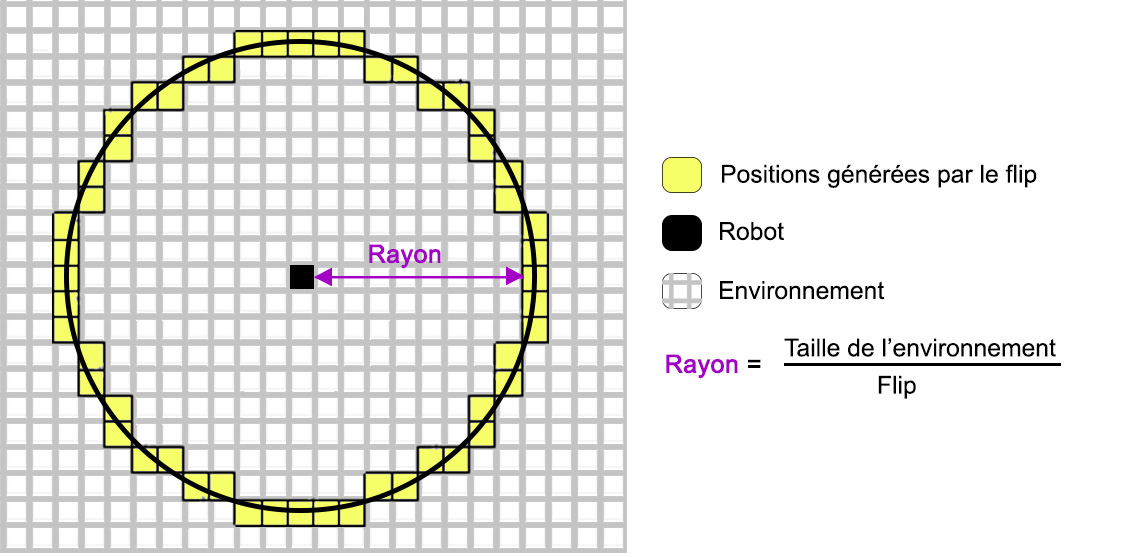
\includegraphics[width=0.7\textwidth]{flip.jpg}%
	\vspace{-0.1 cm}
	\captionof{figure}{Représentation de la méthode de génération de solutions avec le flip.}\label{flip}%
\end{center}



\subsection{MaxChance}
Une solution possède un nombre maximum de chances pour être sélectionnée comme solution de référence. Ce paramètre est aussi exploité afin de détecter la stagnation.

\subsection{Table Dance}
À chaque itération les abeilles déposent leurs meilleures solutions dans une table appelée \textit{"Table Dance"}. Cette table sera exploitée pour choisir la solution de référence de la prochaine itération. Ce choix se fait selon l'un des deux critères suivants:

\subsubsection{Critère de qualité (Best In Quality)}
Parmi les solutions présentes dans la table \textbf{Dance}, la meilleure en termes de qualité est celle possédant la valeur la plus élevée après évaluation.
Un exemple de sélection de la meilleure solution est illustré dans la figure \ref{bestQ} suivante:

\begin{center}	  
	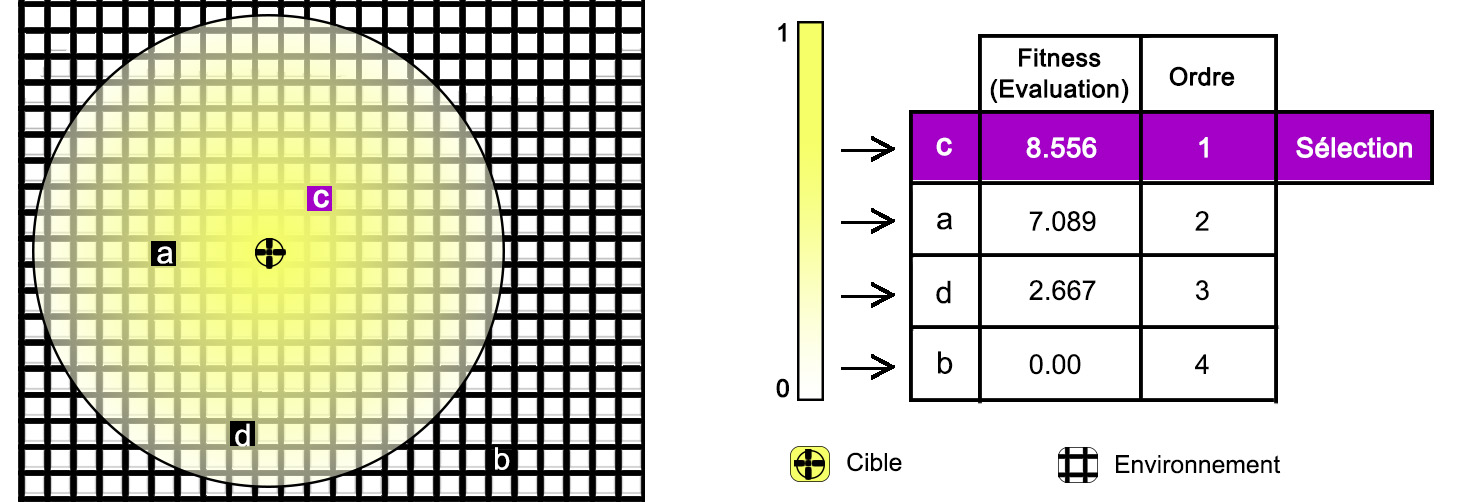
\includegraphics[width=0.85\textwidth]{BestQuality.jpg}%
	\vspace{-0.1 cm}
	\captionof{figure}{Méthode de sélection de la meilleure solution en termes de qualité.}\label{bestQ}%
\end{center}

\subsubsection{Critère de Diversité (Best In Diversity)}
En cas de stagnation, BSO  a recours au choix de la meilleure solution en termes de diversité appartenant à la table \textit{Dance} et ne figurant pas encore dans la liste \textit{Tabou}. Ce mécanisme permet l'exploration des zones distantes tout en évitant de tomber dans un minimum local.

Pour cela nous devons calculer la distance entre deux solutions, la formule choisie est la distance euclidienne, donnée comme suit:
\begin{equation}
Distance(S_1 , S_2) = \sqrt{(x_1 - x_2)^2 + (y_1 - y_2)^2}
\end{equation}

$S_1 :$ Solution 1 avec coordonnées ($x_1 , y_1$)

$S_2 :$ Solution 2 avec coordonnées ($x_2 , y_2$)\\

Le choix de la solution la plus diverse se fait en sélectionnant la solution dont la distance minimale par rapport aux autres solutions est maximale.
Cette méthode de sélection est schématisée dans la figure \ref{bestD} ci-contre:

\noindent
\begin{center}	  
	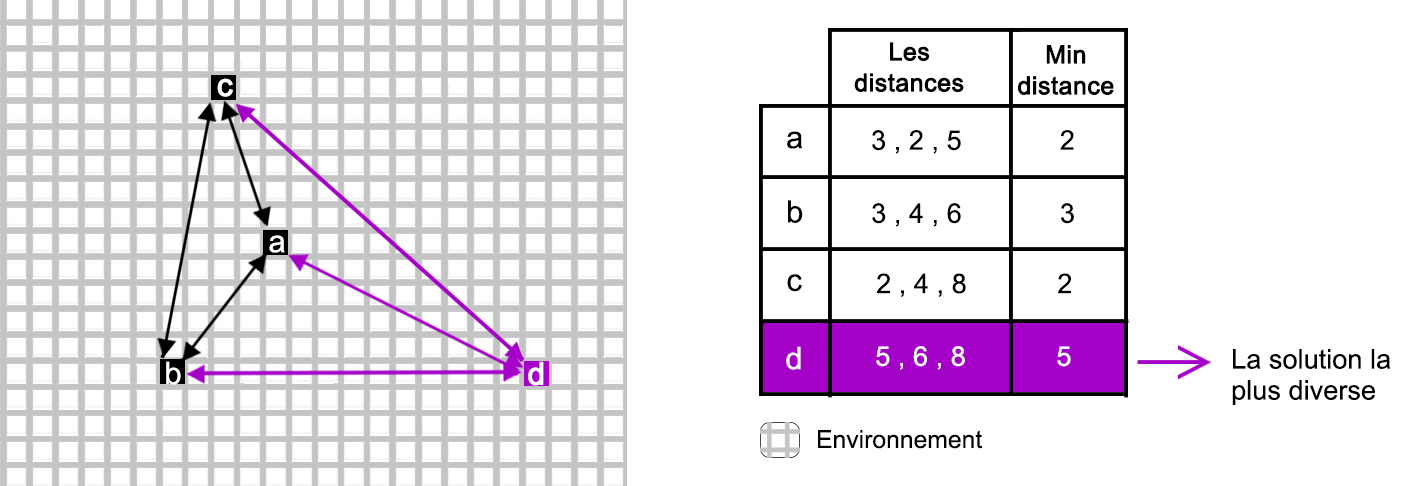
\includegraphics[width=0.9\textwidth]{BestDiversity.jpg}%
	\vspace{-0.1 cm}
	\captionof{figure}{Méthode de sélection de la meilleure solution en termes de Diversité.}\label{bestD}%
\end{center}




\textbf{ }\\

%\newpage

\section{Fonctionnement du Mono-BSO}
L’approche Mono-BSO est constituée d’un seul essaim d’abeilles où chaque robot se comporte comme une seule abeille. Les différentes étapes du Mono-BSO pour la recherche de cibles sont détaillées dans ce qui suit, suivi d'un organigramme \ref{monoBSO} résumant ces derniers.



\subsection{Initialisation de la solution de référence (Sref)}
Une solution (position(\textit{x,y})) est générée aléatoirement et conformément aux contraintes énoncées dans notre modélisation (voir section \ref{sol}).

\subsection{Insertion de Sref dans la liste \textit{Tabou}}
\label{etape2}
La solution de référence (Sref) de l'itération courante \textit{"t"} sera mise dans une liste \textit{Tabou} qu'on définit comme suit:
\paragraph{Liste Tabou }
Lorsqu'une position a déjà servi pour une abeille, nous gardons trace son passage dans la liste \textit{"Tabou"}, cela permet  de réduire la redondance (passage par les mêmes positions).  

\subsection{Génération des zones de recherche}
À partir de la solution de référence (Sref) on génère d'autres solutions, ces dernières déterminent des zones équidistantes de Sref. La génération de ces zones de recherche se fait grâce à l'opérateur \textbf{Flip}. 

\subsection{Affectation des zones aux abeilles}
Une fois les zones générées, on les affecte aux \textbf{"nbrBees"} abeilles de l'essaim de façon à ce que chaque abeille soit responsable de sa propre zone. 

\subsection{Recherche locale pour chaque abeille} 
Chaque abeille effectue une recherche locale qui consiste en l'évaluation d'une surface ronde de l'environnement dont le rayon est de vingt cases, cela constitue l'étape d'intensification. 

Dans le cas où la recherche locale apporte une amélioration, l'abeille prend cette nouvelle solution et réitère ce processus jusqu'à l'absence d'amélioration.

\subsection{Déplacement des abeilles}
Lors de la recherche locale, les abeilles peuvent trouver de meilleures solutions que celles qui leur ont été affectées, c'est pourquoi elles se déplacent vers ces solutions plus prometteuses dans l'environnement, ce qui simule le déplacement du robot. Chaque déplacement d'une position à une autre se fait à travers notre stratégie d'évitement d'obstacles (stratégie d'échantillonnage).


\subsection{Insertion des meilleures solutions dans la table \textit{Dance}}
Lorsqu'une abeille termine sa recherche locale elle communique sa meilleure solution au reste de l'essaim, cela en l'inscrivant dans la table \textit{Dance} commune à l'essaim.

Lorsqu'une cible est atteinte on incrémente le compteur relatif au nombre de cibles trouvées, si le nombre objectif de cibles \textbf{"nbrCible"} est égalé, la recherche prend fin avec succès.


\subsection{Choix de la nouvelle Sref}
Si à l'itération courant \textit{"t"} le nombre de cibles recherchées n'est pas atteint, une nouvelle solution de référence doit être choisie pour la prochaine itération.
 
Il existe alors deux critères possibles, le critère prioritaire est celui de qualité. 
Une solution prise selon le critère de qualité peut demeurer comme Sref au fil des itérations pour un nombre \textbf{"MaxChances"} de fois.
Dans le cas où toutes les chances données à cette Sref sont épuisées (stagnation), le choix de la nouvelle Sref se fera selon le second critère, celui de diversité.



\subsection{Critère d'arrêt de la recherche}
BSO continuera de réitérer les étapes citées plus haut à partir de \ref{etape2} jusqu'à à atteindre le nombre maximum d'itérations \textbf{"MaxIter"} ou le nombre de cibles recherchées \textbf{"nbrCible"}.



\paragraph{Remarque:}
Contrairement aux autres méta-heuristiques, BSO n'utilise pas seulement la fonction d'évaluation comme critère de sélection de solution, mais aussi la diversité. C'est un mécanisme pour remédier au problème de stagnation dans les minima locaux.



\noindent
\begin{center}
	\captionsetup{width=1\linewidth}
	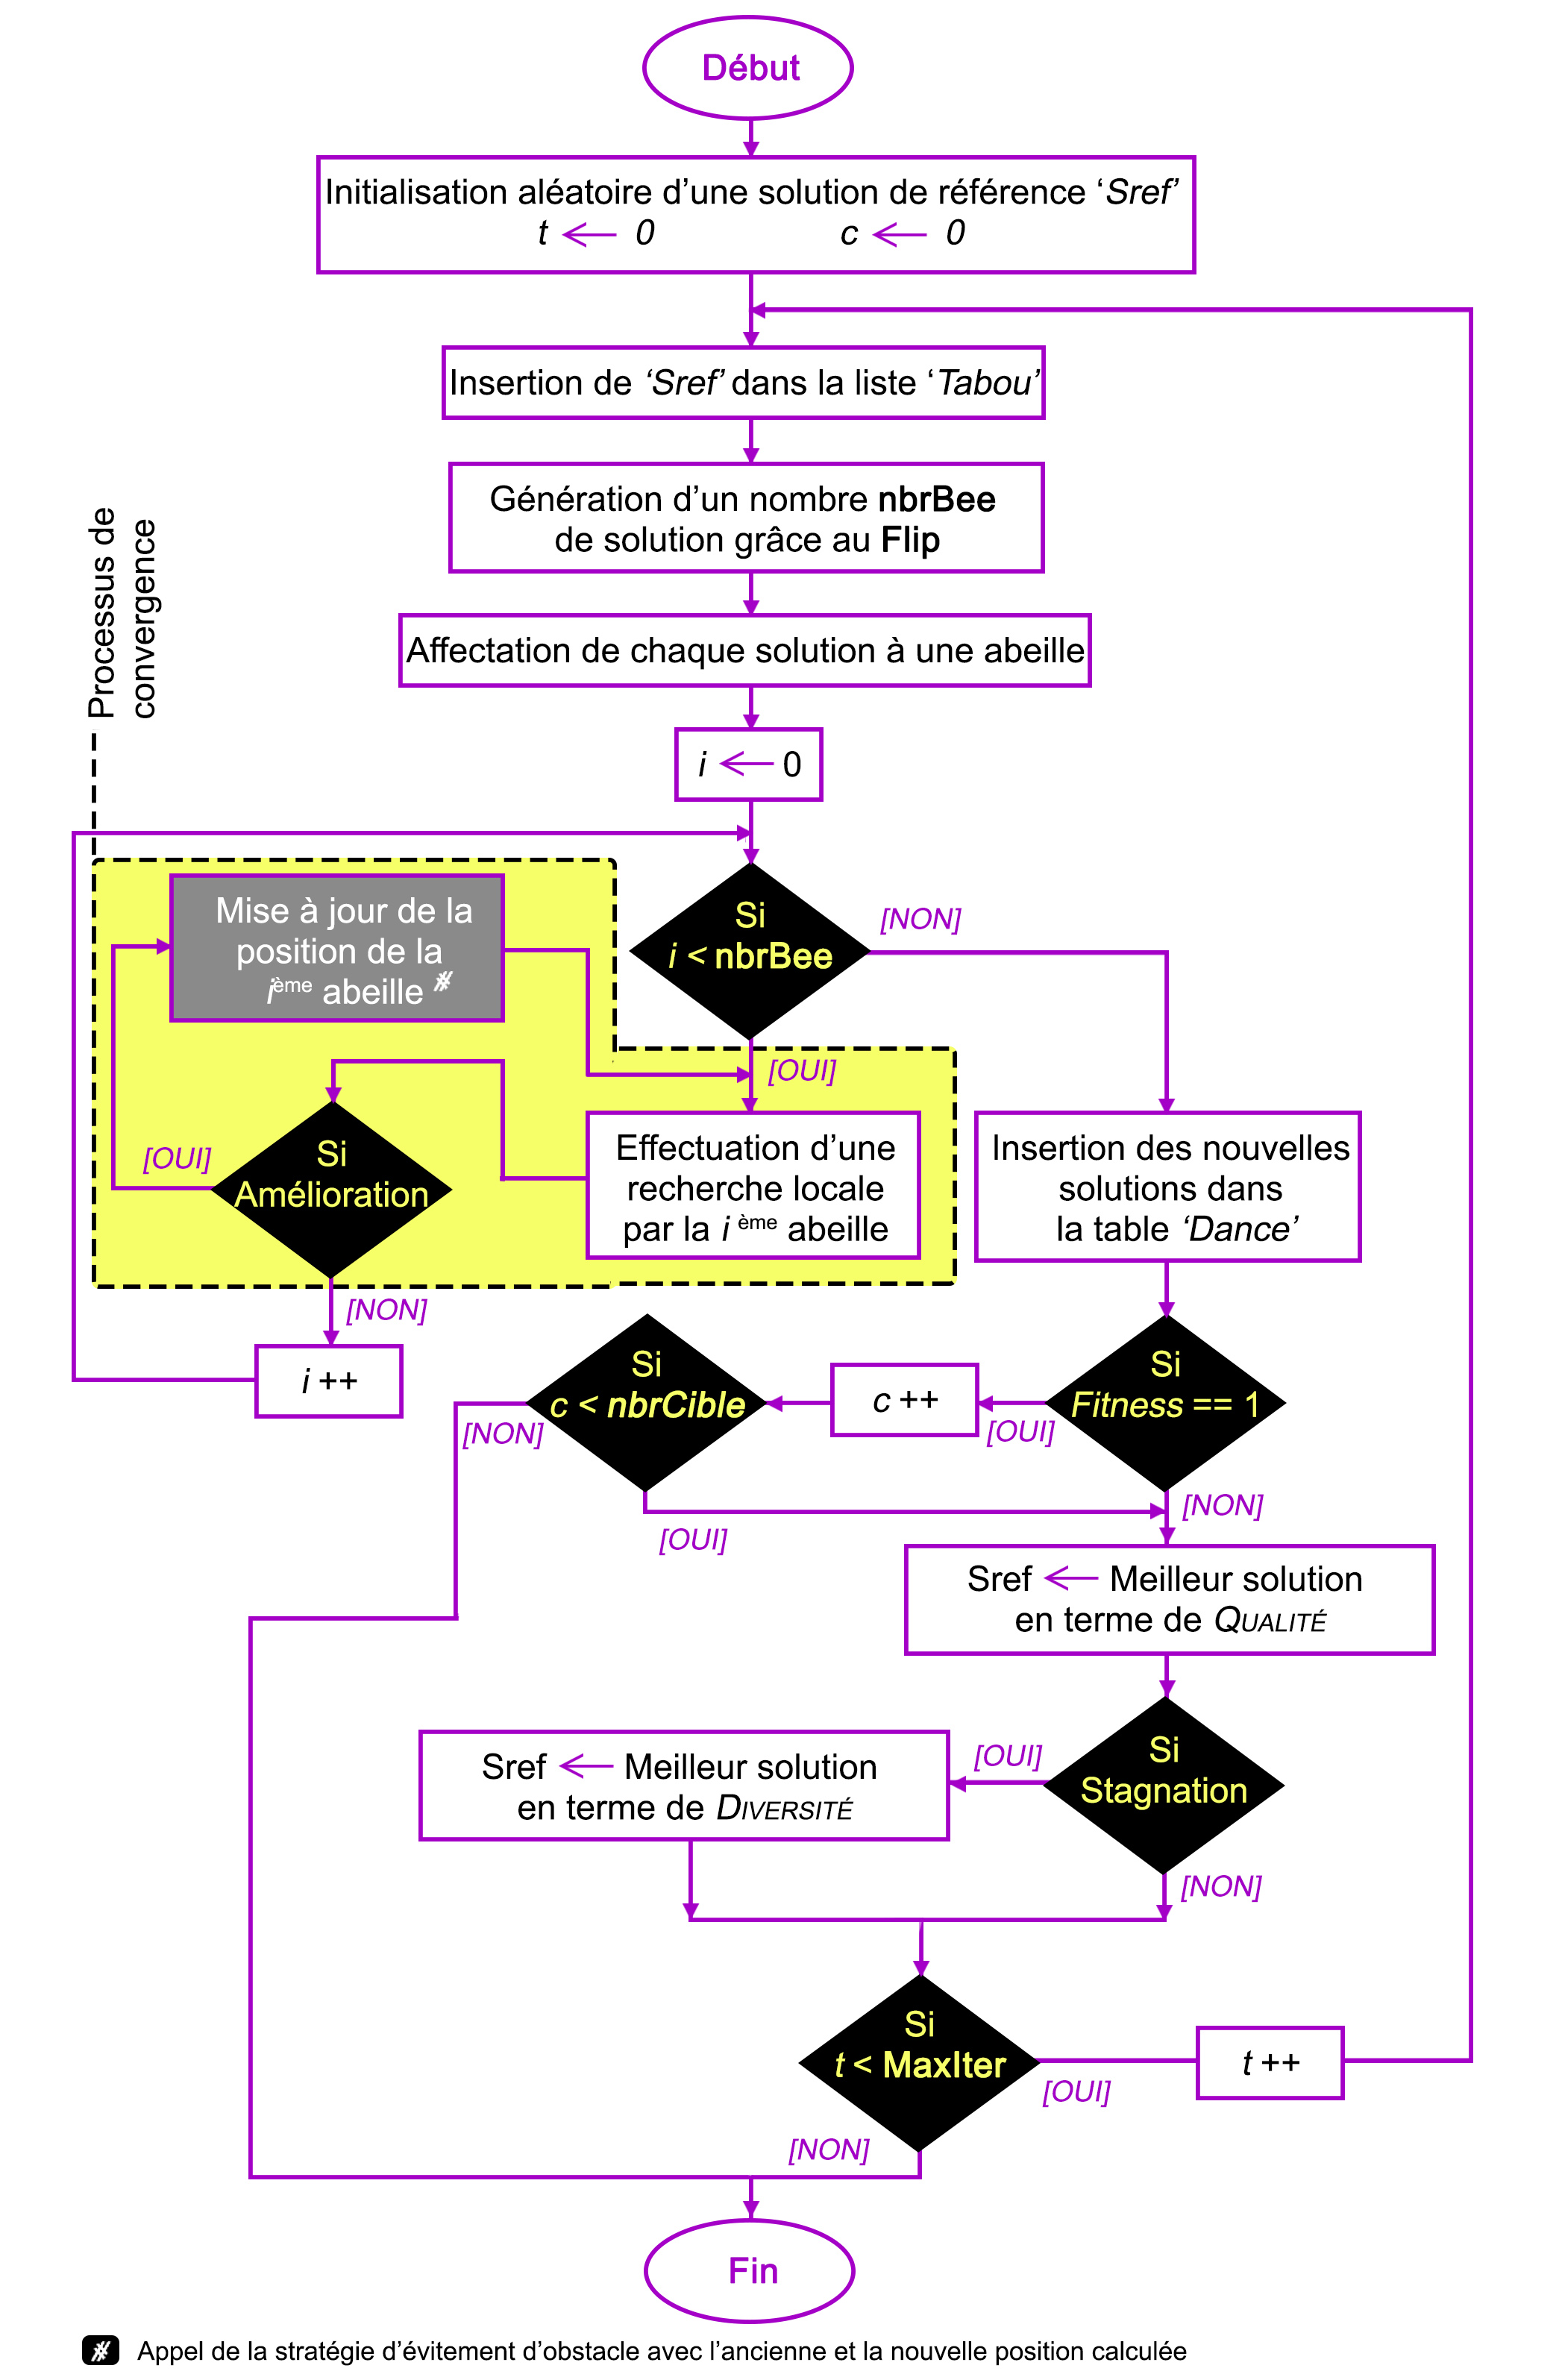
\includegraphics[width=1\textwidth]{mono-bso.jpg}%
	\vspace{-0.1 cm}
	\captionof{figure}{Organigramme du mode de fonctionnement de l'approche mono-BSO.}\label{monoBSO}%
\end{center}

\newpage

\section{Fonctionnement du Multi-BSO}
L’approche Multi-BSO quant à elle, consiste à associer à chaque robot, un essaim d’abeilles. Ils sont donc indépendants les uns des autres, mais ils sont en mode de coopération pour la recherche des cibles. Ils suivent le modèle d’interaction du tableau noir des systèmes multi-agents. Le processus de recherche de cibles implémenté à l’aide de Multi-BSO est décrit dans ce qui suit :

\subsection{Initialisation des solutions de référence (Srefs)} 
Un nombre \textbf{"nbrSwarm"} de solutions (x,y) est généré aléatoirement dans l'espace des solutions, de telle sorte à respecter les contraintes citées dans notre modélisation (voir section \ref{sol}).
Chaque position Sref est attribuée à un robot.


\subsection{Insertion de Sref dans la Liste Tabou}
Chaque essaim d'abeilles relatif à un robot dépose sa solution de référence (Sref) dans la liste \textit{Tabou}. Cette Liste \textit{Tabou} est commune à tous les robots, elle constitue leur moyen de communication (inter-essaim), permettant de réduire la redondance et repassage sur les mêmes solutions.

\subsection{Génération des zones de recherche }
À partir de la solution de référence (Sref) de chaque robot, les zones de recherche sont générées grâce à l'opération de \textbf{"Flip"}. Chaque zone est définie par une position dans l'espace de recherche.

\subsection{Affectation de chaque zone à une abeille }
Pour chaque robot disposant de \textbf{"nbrBees"} abeilles, chaque zone de recherche calculée précédemment est affectée à une abeille de son essaim, celle-ci y prend position.

\subsection{Recherche locale pour chaque abeille}
Chaque abeille effectue une recherche locale à partir de la zone qu'elle s'est vue affectée. Cette recherche consiste en l'évaluation des solutions (positions) de son voisinage à travers la fonction objectif.

À noter que tant qu'une abeille améliore la qualité de sa solution la recherche locale est réitérée de manière récursive.

\subsection{Insertion des solutions dans les tables \textit{Dance}}
Chaque essaim possède sa propre table \textit{Dance}, celle-ci permet la communication intra-essaim de telle sorte que chaque abeille y insère sa meilleure solution locale (de sa zone), afin d'en informer le reste de l'essaim. 


\subsection{Test de la $1^{\grave{e}re}$ condition d'arrêt}
Si une des abeilles a atteint une cible (solution optimale), le nombre de cibles trouvées \textit{"c"} est mis à jour. 
Dans le cas où le nombre de cibles recherchées \textbf{"nbrCible"} est égalé, alors la mission touche à sa fin.

\subsection{Choix de la nouvelle solution de référence}
À priori, la meilleure solution en matière de qualité est sélectionnée à partir de la table \textit{Dance} comme nouvelle solution de référence (Sref).
Sauf en cas de stagnation où une même solution est prise pour solution de référence au-delà de \textbf{"MaxChances"} fois, Sref est alors choisie selon le critère de diversité.


\subsection{Déplacement des robots}
Chaque robot se déplace de son ancienne position vers la nouvelle position calculée (Sref) en employant notre stratégie d'évitement d'obstacles.


\subsection{Test de la $2^{\grave{e}me}$ condition d'arrêt}
Le nombre d'itérations \textit{"t"} est incrémenté puis comparé au nombre maximum d'itérations \textbf{"MaxItér"} accordé à la recherche.\\



L'approche Multi-BSO peut alors être perçue comme l'application de Mono-BSO par chaque robot. L'organigramme de son fonctionnement est résumé dans la figure ci-contre.
\noindent
\begin{center}	  
	\captionsetup{width=1\linewidth}
	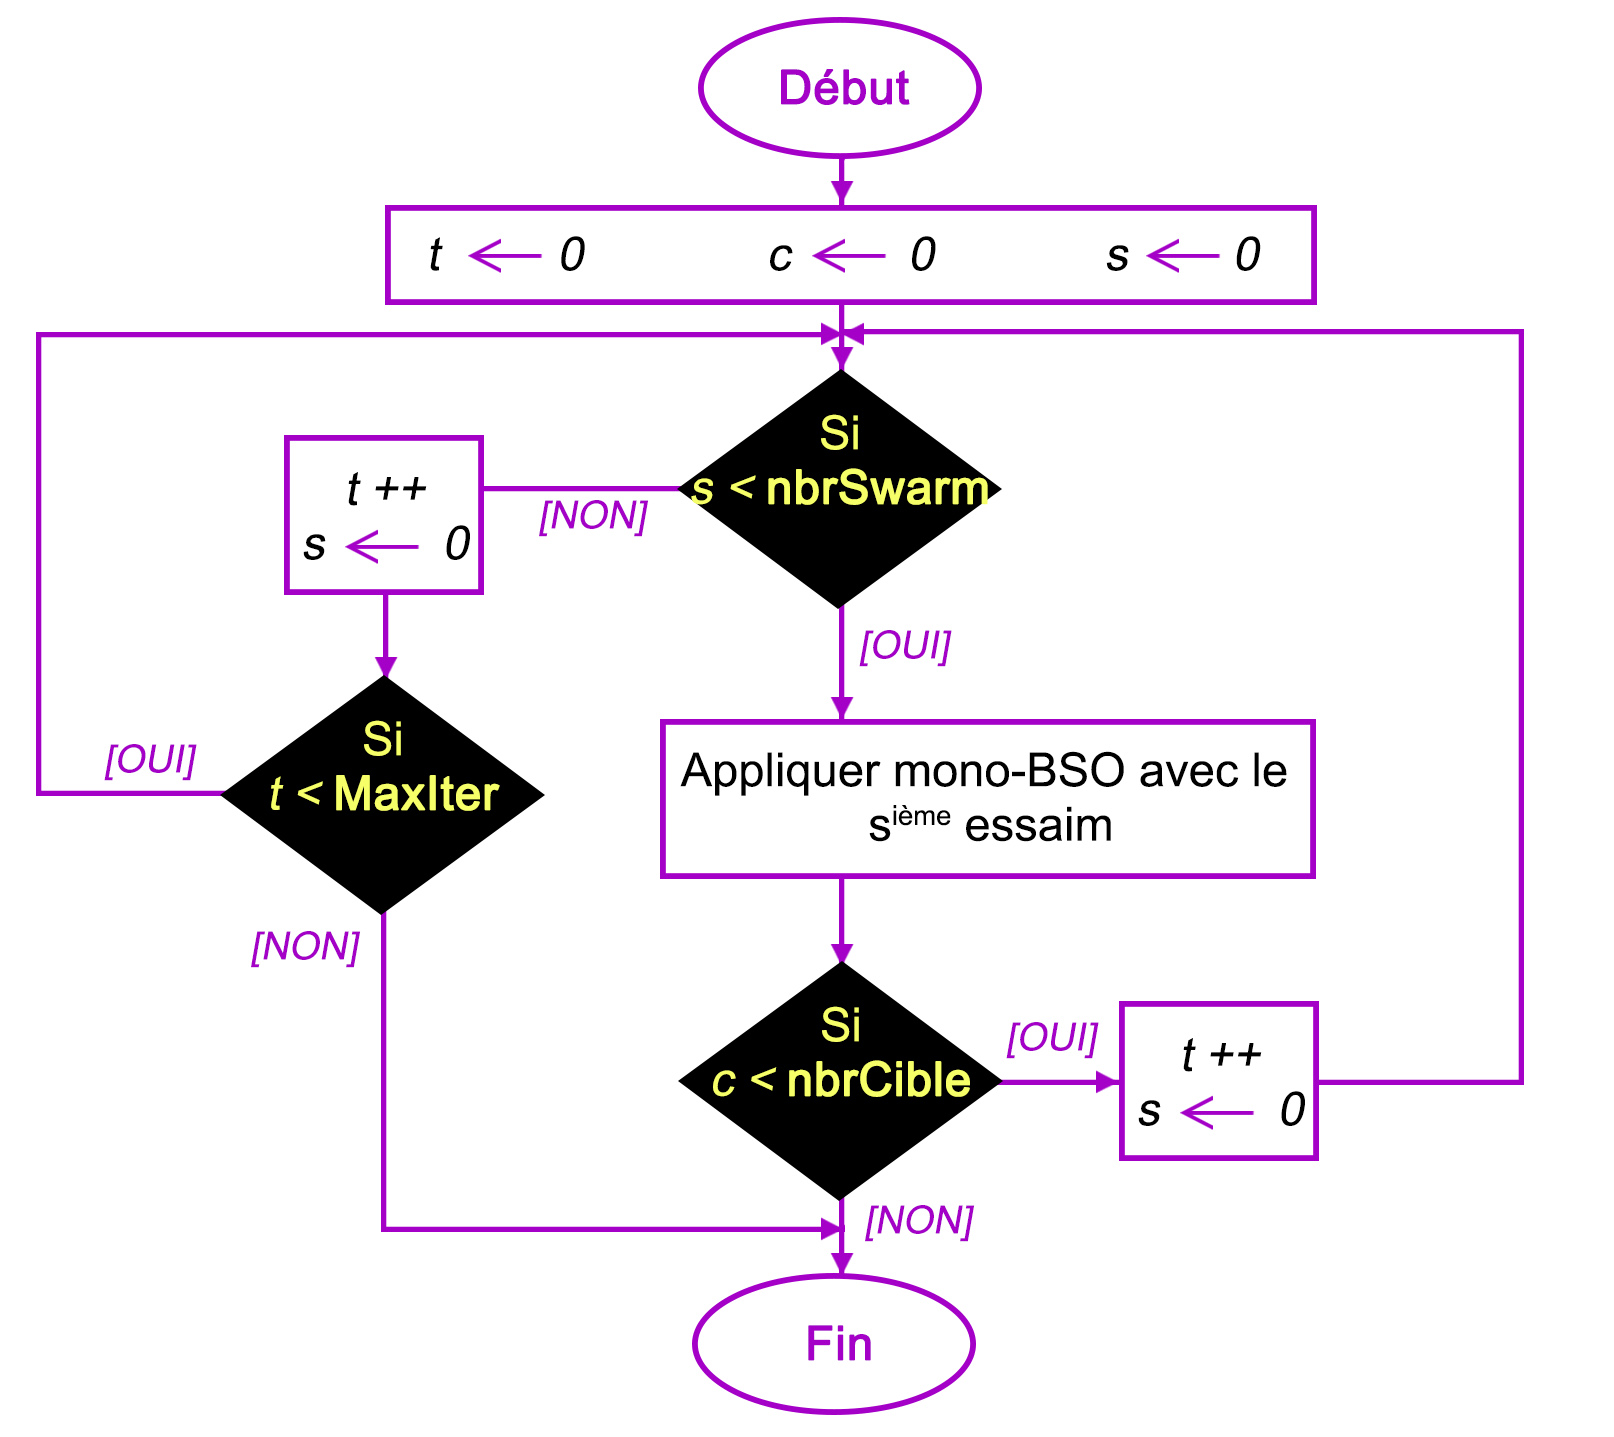
\includegraphics[width=0.7\textwidth]{multi-bso.jpg}%
	\vspace{-0.3cm}
	\captionof{figure}{Organigramme du mode de fonctionnement de l'approche multi-BSO.}\label{multiBSO}%
\end{center}


\section{Conclusion}
À travers ce chapitre, on a pu mettre en évidence deux approches inspirées du comportement des abeilles BSO et Multi-BSO. Ces algorithmes intelligents reposent sur les mêmes paramètres et fonctions de base, mais avec un mode d'emploi légèrement différent pour Multi-BSO qui nécessite la coordination des essaims (équipes) d'abeilles.

Tout en restant dans la même dynamique des techniques inspirées des comportements d'animaux, nous nous penchons dans le chapitre suivant sur deux approches simulant le comportement des éléphants, qui sont très différents des abeilles de part leurs tailles et mécanismes sociaux.






